\documentclass[11pt]{report}

\usepackage{fancyhdr} % Cabeceras de página
\usepackage{lastpage} % Módulo para añadir una referencia a la última página
\usepackage{titling} % No tengo claro para qué es esto
\usepackage[left=3cm,right=2.5cm,top=3cm,bottom=2cm]{geometry} % Márgenes
\usepackage[T1]{fontenc}
\usepackage[utf8x]{inputenc}
\usepackage{xspace}
\usepackage{graphicx}
\usepackage{tikz}
\usepackage{wrapfig}
\usepackage{hyperref}
\usepackage{amssymb}
\usepackage{multirow}
\usepackage[official]{eurosym}
\usepackage{enumitem}
\usepackage{pdfpages}
\usepackage{ifthen}
\usepackage{etoolbox} % Comandos guays.

\hypersetup{
  	hyperindex,
    colorlinks,
    allcolors=blue!60!black
}


\setcounter{secnumdepth}{2}
\renewcommand{\baselinestretch}{1.4}

\title{UAM Software Notification and Damage Management System \\ Fault Manager Lite \\ Risk Management and Planning Document}
\date{\today}
\author{{\Large Triforce} \\ \vspace{5pt} \textit{Iván Márquez Pardo, Víctor de Juan Sanz, Guillermo Julián Moreno}}

\fancyhf{}
\fancypagestyle{plain}{%
	\lhead{\raisebox{12pt}{\textsc{Risk Analysis} - \small Ref. TFC-UAM-01}}
	\chead{\centering \vspace{-15pt} 
\includegraphics[width =40 pt]{Logo.jpg}}
	\rhead{\raisebox{12pt}{\small Ver. 1.0 - \today \vspace{2pt}}}
	\cfoot{\thepage\ of \pageref{LastPage}}
	\rfoot{}
}

\newcounter{risks}[subsection]
\newcommand{\header}[1]{\\ \indent \textbf{#1}\hspace{10pt}}

\newcommand{\reqvertsep}{\vspace{-12pt}}

\newcommand{\riskcat}{\subparagraph{Category}}
\newcommand{\riskdesc}{\reqvertsep\subparagraph{Description}}
\newcommand{\riskprob}[1]{\reqvertsep\subparagraph{Probability} $#1 \%$}
\newcommand{\riskimpact}{\reqvertsep\subparagraph{Impact}}

\newenvironment{risk}[2][]{
	\ifthenelse{\equal{#1}{}}{}{\label{#1}}
	\refstepcounter{risks}
	\subsubsection{Risk \arabic{risks} - #2}
}{}


\newcounter{reqs}[chapter]
\newcounter{NFreqs}[chapter]


\newcommand{\reqdesc}{\subparagraph{Description}}
\newcommand{\reqin}{\reqvertsep\subparagraph{Input data}}
\newcommand{\reqout}{\reqvertsep\subparagraph{Output data}}
\newcommand{\reqsteps}{\reqvertsep\subparagraph{Steps}}

\newenvironment{requirement}[1]{
	\refstepcounter{reqs}
	\par {\noindent \bfseries {\textsc{Functional Requirement \arabic{reqs}} - #1}} \par
}{\vspace{20pt}}

\newenvironment{NFrequirement}[1]{
	\par {\noindent \bfseries {\textsc{Non-Functional Requirement \arabic{NFreqs}}}} \par
	\refstepcounter{NFreqs}
}{\vspace{20pt}}

\newcommand{\reqref}[1]{Req. \ref{#1}}



\makeindex

\begin{document}
\maketitle
\tableofcontents
\newpage
\chapter{Introduction}


\label{chapIntroduction}

The Autonomous University of Madrid (UAM) has reported the numerous problems it has detecting faults that arise on its campus and its facilities, whose reparation usually takes excessive time and is poorly organized. A late detection of faults in the facilities delays its reparation, stopping its users to continue using them as normal and complicating the maintenance staff labor. Regarding the wishes of the campus users and realizing the potential maintenance problems it has, the UAM has organized a contest to choose the best project proposal that solves them.

This is where our organization, Triforce, enters the scene: we have analyzed the problem exhaustively and designed a web application, Fault Manager Lite (FML), that meets all the requirements expected, solves the problems and also includes new extra features that makes it even more useful.

\section{Purpose}

The purpose of this Project Plan document is to provide a detailed description of the requirements for the project and estimations of the size of the whole system. Based on these aspects, we introduce our proposed planning for the development, including related estimates such as cost and duration.

The intended audience of this document is the executive team of Triforce, in order to know and evaluate the resource allocation for the project and its fit in the company and its activities.

\section{Structure}

The document is structured as follows. This chapter serves as introduction and description of the document and its contents.

Chapter \ref{chapReferences} contains the references used to define, analyze and estimate risk.

In chapter \ref{chapDef} we review the project definition and the subsystems it has.

Our planned schedule and cost estimations is presented in chapter \ref{chapPlan}. We also include some important requirements of the project.


Finally, chapters \ref{chapRiskAnalysis}, \ref{chapRiskManagement} and \ref{chapRiskMonitoring} includes the analysis (identification and estimation) of the risk in FML project, how we plan to management them and finally the monitoring process we will use to ensure the risk don't arise.

The appendices contain extra information, such as the riskology tool (appendix (\ref{chapRiskology}and the detailed Gantt diagram (appendix \ref{chapGantt}).

\section{Scope}

The final goal of the system we want to develop is integrating in a single application an user-friendly report system of faults on the facilities of the UAM campus with an efficient repair task manager for the maintenance staff of the UAM. Moreover, the application will provide statistics of the reported faults and will count with extra features such as a notification and messaging system which may serve as a communication channel between campus members and campus technicians.

What makes this system unique and useful for the UAM is the union of different features (report system and task management) from other applications, but specially designed taking into account the UAM's maintenance service current needs. More information and exhaustive analysis about other similar applications can be found in Fault Manager Lite SRS[1].

Other main goal of the application is the equalization of the working way of the different departments of the maintenance service. Nowadays they are self-organized and they lack of much coordination, which leads to a continuous loss of time in the troubleshooting of faults. Therefore, this application aims to substitute the organization methods of the different maintenance departments.

Fault Manager Lite will use the UAM's authentication system in order to access the application; therefore, it will not substitute the current authentication system nor store in its own database any UAM's credentials. However, the application will have its own users database in order to properly manage them inside its limits (i.e. for banning or messaging reasons).

The requirements analysis contained in this document has two fundamental objectives: the first one, to serve as a first version for its valoration by the client company (in this case, the UAM), who will be able to specify if they want any extra functionality or, on the contrary, they want to quit any of the extracted requirements; the other one, it will be used as a basis for the system size estimation that will let us know the approximate duration, personnel needed and expected costs of the project. Therefore, the requirements are not definitive in any way, and can be extended or modificed in the analysis phases that will be performed during the development.

The project plan obtained from the estimations will be the one used if the direction of Triforce approves the estimated costs and duration as long as the client doesn't ask for changes on the requirements that can cause great variations in the estimated effor. On the contrary, a new version of the project plan that considers the new conditions will be needed.

\section{Responsibilities}

For FML project organization purposes, a several charges of responsibility have been designated as seen in Table \ref{tbl_Responsibilities} depending on the perfomance and abilities shown in previous projects developed in Triforce.

Each one of these responsibles will be in charge of the management and coordination of its dedicated section, as well as the communication with other sections implied in the project.


\begin{table}[hbtp]
\centering
\begin{tabular}{|c|p{5cm}|} \hline
\textbf{Project Leader} & Guillermo Julián Moreno \\ \hline
\textbf{Project Head} & Víctor de Juan Sanz \\ \hline
\textbf{Project Quality Manager} & Iván Márquez Pardo \\ \hline
\textbf{Project Documentation Manager} & Guillermo Julián Moreno \\ \hline
\textbf{Customer Representative} & Víctor de Juan Sanz \\ \hline
\end{tabular}
\caption{People in charge of the FML project.}
\label{tbl_Responsibilities}
\end{table}

\section{Definitions}

This section gathers the terms and abbreviations used along this document.

\emph{FML: } Fault Manager Lite, the application whose development we are planning in this document.

\emph{UAM: } Universidad Autónoma de Madrid, the client who has requested the development of the application.

\emph{FP: } Function Points.

\emph{UFP: } Unadjusted Function Points.

\emph{AF: } Adjusting Factor.

\emph{AFP: } Adjusted Function Points.

\emph{Person-day: } Estimation of effort given by FP.


\section{Reference Documentation}
\begin{table}[hbtp]
\centering
\begin{tabular}{|c|p{10cm}|} \hline
\textbf{Reference} & Title \\ \hline
1 & Fault Manager Lite Software Requirements Specification \\ \hline
2 & \url{http://csse.usc.edu/csse/research/COCOMOII/cocomo2000.0/CII_modelman2000.0.pdf} \\ \hline
\end{tabular}
\end{table}

\chapter{References}
\label{chapReferences}
\chapter{Project definition}
\label{chapDef}
% -*- root: ../ProjectPlan.tex -*-
\section{Project Definition}

FML is based on the jolly cooperation between the users of the facilities of the UAM campus and the maintenance staff in charge of them.

As the users will be the ones that will detect the sooner faults on the facilities the campus offers them, they are also the most suitable to report the problems they are having, in order to getting them fixed as soon as possible. With the FML web application, it will only take less than a minute to fill the form and send it to the maintenance staff.

Using the reports of faults detected in the campus, the maintenance personnel will stop losing its precious time revising the installations looking for faults and will be able to focus on the repairs. Apart from this benefit, the maintenance staff will also have a better way to coordinate efforts, as the FML will provide an automatic assignment system to assign repairs to each of the members avoiding overloading any of them and taking into account their distance to the problem, saving time on displacements.

In summary, the users will be able to easily report faults on facilities they are using in order to have them fixed in the less time possible, while the maintenance personnel will multiply its current performance as the majority of their resources will stop being wasted on revisions, but on repairs. 

\section{Breakdown in Subsystems}

\begin{figure}[hbtp]
\centering
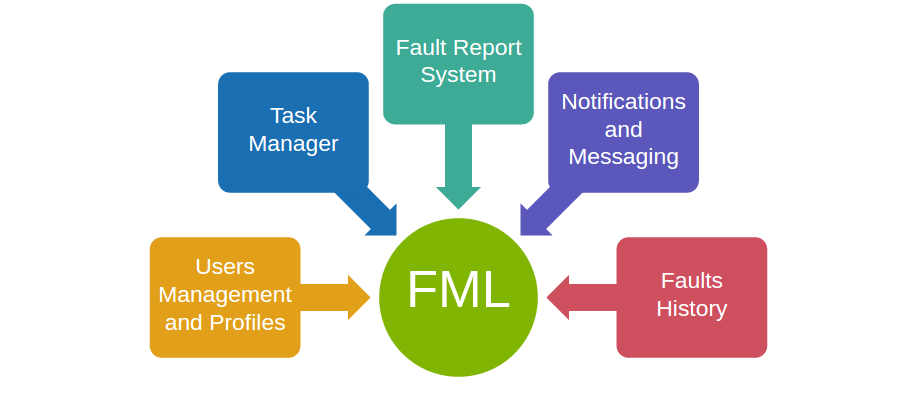
\includegraphics[scale=0.5]{img/subsystems.png}
\caption{Schematic for the subsystems of the project.}
\label{figSubsystems}
\end{figure}

In order to achieve the goals described in chapter \ref{chapIntroduction}, the Fault Manager Lite application is divided into five subsystems: \emph{Task Management}, \emph{Report System}, \emph{Notification and Messaging System}, \emph{User Management} and \emph{Faults History and Statistics}, as seen in figure \ref{figSubsystems}.

A brief description of the functionalities of each mentioned subsystem can be found in the next sections of the document.

\subsection{Task Management}
\label{subsection Task Management}

This subsystem is in charge of the management of repair tasks, which are automatically generated whenever the system receives a new fault report.

Users will use the report system of the application (see \ref{subsection Report System}) to send report faults. These faults will be analyzed by this subsystem and automatically classified depending on their department and priority. Then, their corresponding repair task will be generated based on the form filled by the user and assigned to the closest technician depending on the location of the fault.

Managers will be able to change manually the priority and the person in charge of repairing that fault, which are automatically assigned by the subsystem. The category of the fault can also be modified in case it is not correct; in that case, the fault will then be sent to the manager of the new department. Cleaning department will be treated differently as there is a manager for each building of the UAM campus, so cleaning tasks will be assigned to those managers taking into account this characteristic.

Technicians who have been assigned a repair task will be notified (see \ref{subsection Notification and Messaging System}) and be able to consult the information related to that task. This task information includes: ID of the reporter, location of the fault, timestamp of the report, brief description (subject), detailed description, category, status, priority and occasionally a photography (if any was given by the reporter).

The status of a fault can be: \emph{Pending} (just received by the system, before having been automatically assigned by the system or manually assigned by a manager), \emph{Assigned} (already assigned to a technician, who is or will be eventually solving it) or \emph{Solved} (the task has been successfully completed as the fault has been repaired). Technicians will be able to change the current status of a task assigned to them in order to give managers real-time information about the status of faults' troubleshooting.

Managers will also be able to consult real-time information about repair tasks assigned to members of their departments and make reassignments of tasks in case, for example, of overloading a certain technician or in order to accelerate an specific repair.

\subsection{Report System}
\label{subsection Report System}

This subsystem is in charge of the fault report system, which is the main and most important activity of the whole software system.

Whenever users and/or technicians encounter a fault on the facilities of the campus, they will be able to fill a form in order to report that fault and accelerate its troubleshooting. This fault will then be sent to the FML server, which will assign its repair task to the corresponding technician (see \ref{subsection Task Management}).

The mandatory fields of the form include: a brief description of the problem (subject), a more detailed description (1000 characters maximum length), category (department of the maintenance service) and location (which can be automatically set using GPS technology or manually set by the user in case the GPS function doesn't work properly). The ID of the reporter and the timestamp of the report will be automatically added before sending it.

As an optional field, users can add a photography to their report in case they want to be more specific. The photo will be taken on the fly or added from the user's gallery.

After sending a fault report, the reporter will be able to consult the real-time status of its repair task by selecting that task from his/her fault history (see \ref{subsection Fault History and Statistics}). Reporting a fault enables the opening of a chat conversation with the technician assigned to the repair (see \ref{subsection Notification and Messaging System}).

The report system is also in charge of analyzing newly received fault reports and determine if they can be duplicates of existing reports, by comparing their characteristics: location, similar timestamps and same keywords in the descriptions. Potential duplicates will be sent to the manager, who will decide if they really are the same issue or not.

\subsection{Notification and Messaging System}
\label{subsection Notification and Messaging System}
This subsystem is the one in charge of sending and receiving notifications and messages from the application.

There will exist general and emergency notifications (such as special events in the campus and a fire or blackout in a building, respectively). This notifications will only be sent by managers and all the users will receive that alerts.

Technicians will receive a notification informing them of their assignment of a new task. They will also be able to establish a communication channel (private chat) with the reporter of a fault, in order to ask for more information about that fault. Users will not be able to open this communication channel with the technician in charge of their reported fault, while managers will be able to open a private chat with any member of their departments for a better management and organization of them.

When a fault is repaired and the technician changes its status to solved (see \ref{subsection Task Management}), its reporter will receive a notification about the finish of the repair.

Users and technicians will be able to delete messages or notifications they have received.

\subsection{User Management}
\label{subsection User Management}

This subsystem is in charge of several issues related to the application users, including login, user profile and user's fault history.

In this section, the term `user' will make reference to every member of the UAM that uses the FML application as a reporter or as a member of the maintenance service.

When entering the application, users must introduce their credentials for accessing the UAM's web services. Those credentials will be sent to the UAM members server, which will inform the FML server about the correctness (or not) of them. Login credentials will only be needed once (the first time you access to the application).

Every user will have a profile, including some (optionally filled) information about them. From this profile, every user will have access to their fault report history; every report can be selected in order to see its current status (see \ref{subsection Fault History and Statistics}).

In case of students, this profile will also show them information about their current progress in the achievement of optional credits as a reward for their report history.

This system is also in charge of filtering and/or searching for users in the database. This ability to look for users in the database is only accessible to managers.

\subsection{Fault History and Statistics}
\label{subsection Fault History and Statistics}

This subsystem is in charge of several activities related to fault reports, including their search and the generation of statistics related to them.

When a fault is reported (see \ref{subsection Report System}), that report is saved in the database and its entry can be eventually change. For example, its status will be eventually changed when it gets repaired by a technician, it can be assigned to another technician or its priority can be modified by a manager (see \ref{subsection Task Management}).

Managers will be able to consult the fault database to look for all its entries or apply some filters to look for specific faults. Among the filters that can be applied in the search, there are: category/department, date range, reporter, technician or keyword in the description.

User profiles will make accessible information about fault reports related to those users: reporters will see the faults they have reported and their real-time status, while technicians will see the faults they have repaired or have been assigned to do so. Managers will have all this information available by applying the corresponding filter.

Managers will also be able to generate statistics based on the fault history contained in the database. This statistics can be general, related to their departments or related to a member of their technical staff. The generated statistics can be used to analyze the troubleshooting efficiency of the maintenance service or detect problematic areas.

Users will be able to see a simplified map of the campus with colored signs on it. Each dot represents a reported fault and the color will follow a color code, making its status easily distinguishable depending on it: Pending to assign (red), Assigned (yellow) and Solved (Solved). Only the last 30 reports will be shown in this map at the same time to ensure their visibility.




\chapter{Estimation, Planning and relevant requirements}
\label{chapPlan}
% -*- root: ../ProjectPlan.tex -*-
\section{Time estimation and Schedule}
\label{secTimeEstimation}
\subsection{Gantt diagram}

\begin{figure}[hbtp]
\centering
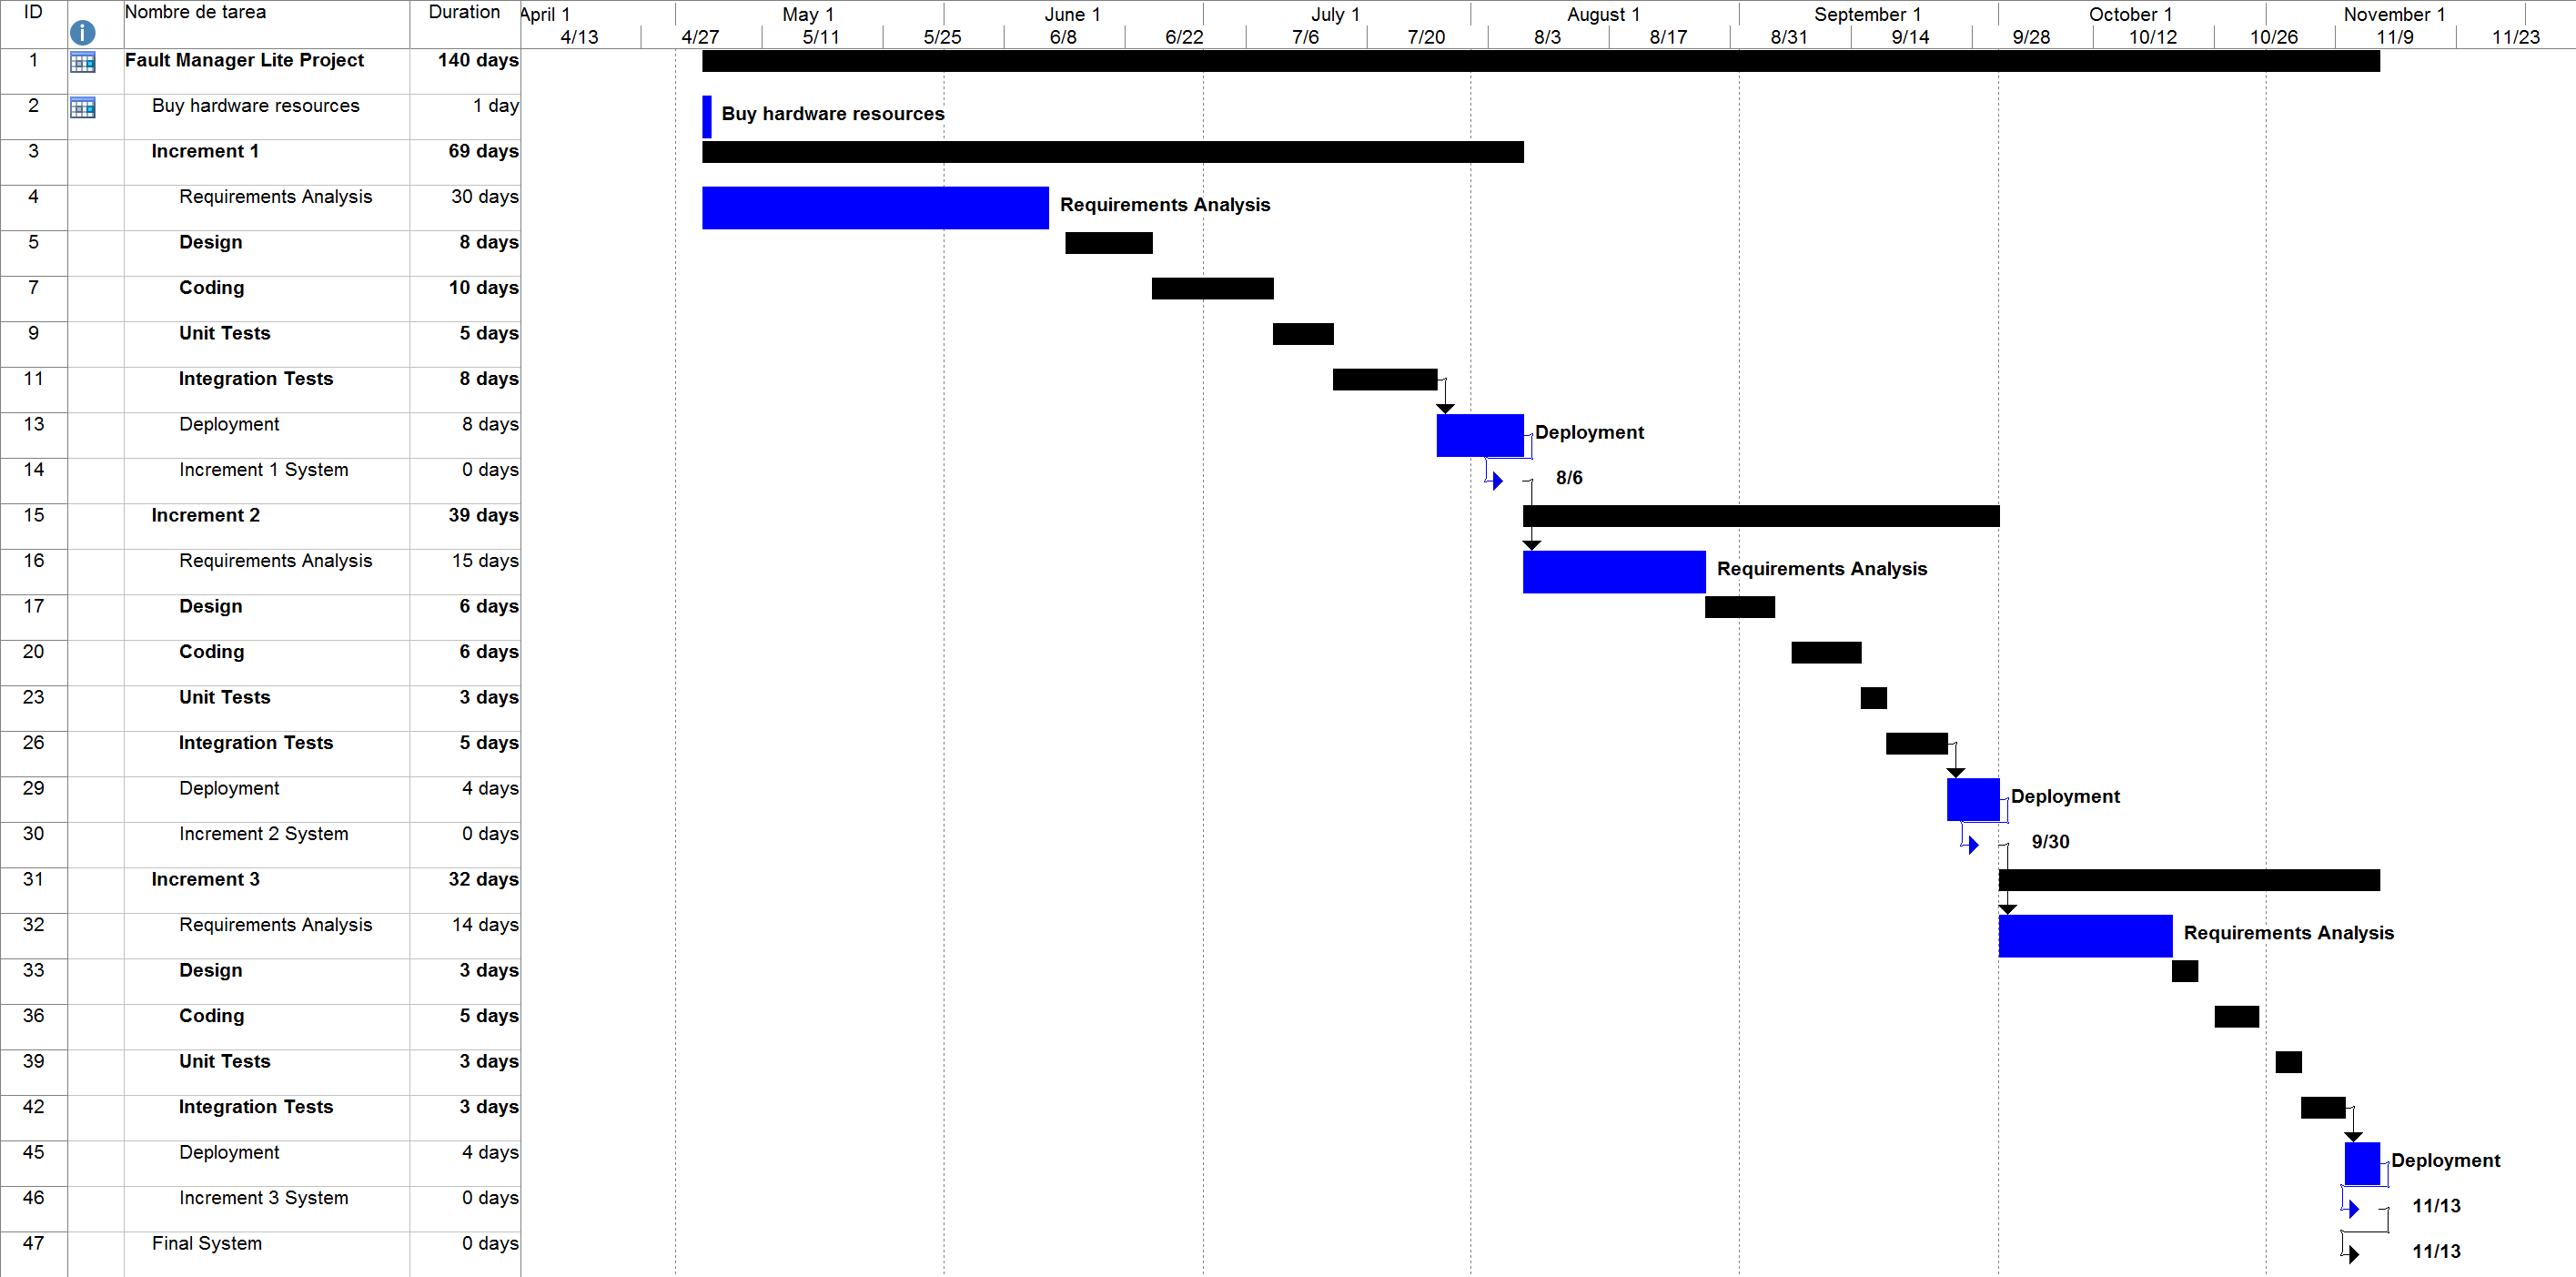
\includegraphics[width=0.8\textwidth]{img/GanttDiagram.png}
\caption{Simplified Gantt diagram.}
\label{figGanttSimple}
\end{figure}

Figure \ref{figGanttSimple} shows a simplified view of the Gantt diagram that represents the schedule of the project. A detailed version of this diagram is included in appendix \ref{chapGantt}.

\subsection{Increment planning}

We have decided to break down the development in 3 increments, each one dedicated to various subsystems. The details of the function points assigned to each increment and the corresponding effort is detailed in table \ref{tblIncrementsSubsystems}. Table \ref{tblSubsystemsAssignedIncrement} reflects the increment in which each subsystem will be completed and the corresponding percentage of each increment's effort dedicated to it.

This is the old detailed estimation of effort in terms of function points.

\begin{table}[hbtp]
\centering
\begin{tabular}{c|l|c|c}
\textbf{Increment} & \textbf{Subsystems} & \textbf{Function Points} & \textbf{Effort (person-days)} \\ \hline
Increment 1 & Task management & 102.3 & 149.972 \\
Increment 2 & Report System, Fault History & 50.6 & 74.213 \\
Increment 3 & Notification and Messaging & 48.4 & 70.986 \\ \hline
\textit{Total} &  & \textit{201.3} & \textit{295.106} \\
\end{tabular}

\caption{Detail of the old increments and corresponding effort.}
\label{tblIncrementsSubsystems}
\end{table}


As the time we had has been limited (10\% less than our initial estimation), we had to remove some system's functionalities. As a result of that process, we have obtained this new detailed estimation of effort in terms of function points.

\begin{table}[hbtp]
\centering

\begin{tabular}{c|l|c|c}
\textbf{Increment} & \textbf{Subsystems} & \textbf{Function Points} & \textbf{Effort (person-days)} \\ \hline
Increment 1 & Task management & 94.6 & 138.6836 \\
Increment 2 & Report System, Fault History & 48.4 & 70.9544 \\
Increment 3 & Notification and Messaging & 37.4 & 54.8284 \\ \hline
\textit{Total} &  & \textit{180.40} & \textit{264.47} \\
\end{tabular}
\caption{Detail of the new increments and corresponding effort.}
\label{tblIncrementsSubsystems}
\end{table}

As we can see in the efforts of each subsystems, they have changed. We have 10\% function points less, so we will finish 10\% earlier. The removed functionalities belonged to the messaging module and to the statistics module, the ones we thought that there were more dispensable. 

In table \ref{tblSubsystemsAssignedIncrement} one can see the effort for each subsystem, and one can corroborate that the affected ones are messaging and statistics.

\begin{table}[hbtp]
\centering

\begin{tabular}{l|c|c}
\textbf{Subsystem} & \textbf{Increment} & \textbf{Effort \%}  \\ \hline
Task Management & 1 & 100 \% \\
Reporting & 2 & 40 \% \\
Notification and Messaging & 2 & 60 \% \\
User Management & 3 & 29 \% \\
Faults History and Stats & 3 & 71 \% \\
\end{tabular}

\caption{Assigned increment and effort for each subsystem.}
\label{tblSubsystemsAssignedIncrement}
\end{table}

Now we include the effort for each phase of each increment in the table \ref{tblIncrementPhases} with its corresponding new effort.

\begin{table}[hbtp]
\centering

\begin{tabular}{|c|c|c|c|}
\hline
\textbf{Increment} & \textbf{Phase} & \textbf{Effort \%} & \textbf{Effort (person-days)} \\ \hline \hline

\multirow{7}{*}{\textsc{Increment 1}} & Analysis & 20 \% & 27.6 \\ \cline{2-4}
& Design & 20 \% & 27.6 \\ \cline{2-4}
& Coding & 20 \% & 27.6 \\ \cline{2-4}
& Unit tests & 10 \% & 13.8 \\ \cline{2-4}
& Integration tests & 20 \% & 27.6 \\ \cline{2-4}
& Implementation & 10 \% & 13.8 \\ \cline{2-4}
& \textit{Total} & \textit{100\%} & \textit{138.6836} \\ \hline \hline

\multirow{7}{*}{\textsc{Increment 2}} & Analysis & 20 \% & 14.20 \\ \cline{2-4}
& Design & 20 \% & 14.20 \\ \cline{2-4}
& Coding & 20 \% & 14.20 \\ \cline{2-4}
& Unit tests & 10 \% & 7.1 \\ \cline{2-4}
& Integration tests & 20 \% & 14.20 \\ \cline{2-4}
& Implementation & 10 \% & 7.1 \\ \cline{2-4}
& \textit{Total} & \textit{100\%} & \textit{70.9544} \\ \hline \hline

\multirow{7}{*}{\textsc{Increment 2}} & Analysis & 20 \% & 10.96 \\ \cline{2-4}
& Design & 20 \% & 10.96 \\ \cline{2-4}
& Coding & 20 \% & 10.96 \\ \cline{2-4}
& Unit tests & 10 \% & 5.4820 \\ \cline{2-4}
& Integration tests & 20 \% & 10.96 \\ \cline{2-4}
& Implementation & 10 \% & 5.4820 \\ \cline{2-4}
& \textit{Total} & \textit{100\%} & \textit{54.8284} \\ \hline

\end{tabular}

\caption{Detail of the increments with the corresponding phases for each one.}
\label{tblIncrementPhases}
\end{table}
% -*- root: ../ProjectPlan.tex -*-
\section{Cost management and resource assignment}

\subsection{Personnel costs}

We consider the following salaries for the required positions for the project:

\begin{itemize}
\item Systems Analyst: 400 \euro / day.
\item Senior Designer: 350 \euro / day.
\item Junior Designer: 200 \euro / day.
\item Systems Technician: 300 \euro / day.
\end{itemize}

These values will be used as the fixed cost for personnel throughout this document estimations, even if they come from SOTFCOM or UAMSOFT.

\subsection{Hardware costs}

For the project, three workstations must be acquired for development (1.650 \euro per unit) and another one for performance testing (3.200 \euro). Total hardware cost is then 8.150 \euro.

Additionally, the maintenance cost for current hardware and software is 1.050 \euro per month.

\subsection{Software costs}

A new integrated development environment will also be acquired, at a cost of 1.100 \euro per workstation. This environment includes all necessary software for the lifecycle of the project.

\subsection{Cost estimation}

Given the schedule detailed in the previous section (\ref{secTimeEstimation}), we present the resource assignment table with the corresponding costs for the whole project in table \ref{tblCostResourceEstimate}. As we can see, the total amount of worked hours is 10\% less than in the previous project plan but the budget is not exactly the 10\% less because of the hardware and workstations needed.

\begin{table}[hbtp]
\centering
\begin{tabular}{r|rr|r}
\textbf{Resource} & \textbf{Quantity} & \textbf{Unit cost} & \textbf{Total cost} \\ \hline
System Analyst & 864 hours & 400 \euro / day & 43,200 \euro \\
Senior Designer & 640 hours & 350 \euro / day & 28,000 \euro \\
Junior Designer 1 & 640 hours & 200 \euro / day & 16,000 \euro \\
Junior Designer 2 & 640 hours & 200 \euro / day & 16,000 \euro \\
Systems Technician & 128 hours & 300 \euro / day & 4,800 \euro \\ \hline
\textit{Total work} & \textit{1,994 hours} & - & \textit{108,000 \euro} \\ \hline \hline
Systems Maintenance & 140 days & 1,050 \euro / month & 7,350 \euro \\
IDE Software & 3 workstations & 1,100 \euro / w.s. & 3,300 \euro \\
Development w.s. & 3 workstations & 1,650 \euro / w.s. & 4,950 \euro \\
Performance w.s. & 1 workstation & 3,200 \euro / w.s. & 3,200 \euro \\ \hline
\textit{Total systems} & - & - & \textit{18,800 \euro} \\ \hline \hline
\textit{Total cost} & - & - & \textit{126,800 \euro}

\end{tabular}

\caption{Cost estimation given the schedule}
\label{tblCostResourceEstimate}
\end{table}

\section{Relevant requirements}
% -*- root: ../RiskAnalysis.tex -*-
We include below the requirements that are relevant to the detected risks.

\subsection{A-1 Notification of incidences}

\begin{requirement}{Fault's location}
\reqdesc Get the location of the fault, based on the location of the reporter.
\reqin Two kind of external inputs are necessary for determine location:
\begin{itemize}
\item Faculty where the fault is located, given by.
\subitem GPS coordinates (if possible).
\subitem Manually chose location.
\item Manually chose floor and room inside the building where the fault is located.
\end{itemize}
\reqsteps Transform input information into Location object.
\reqout Location object.
\end{requirement}

% % % % % % % Req2

\subsection{A-2 Management of priorities}
\begin{requirement}{Definition of priority criteria}
\reqdesc The system must allow to specify different criteria to assign automatically a priority to each incidence.

\reqin The user selects parameters of the incidence object and corresponding keywords that will conform the selection criteria, and the desired priority that will be set on match.

\reqsteps The system stores the criteria and applies it automatically on incidence creation in order to establish a priority.

\reqout The system automatically clasifies each incidence based on user-defined criteria: if a certain parameter (e.g., location or description) contains the keywords specificied, the priority will be set to whatever the user specified in the criteria.
\end{requirement}


% % % % % % Req 3A
\subsection{A-3 Supervision of incidences}
\begin{requirement}{Assign incidences}

\reqdesc Managers of each department will be able to assign the reparation of incidences to technical members of their department.

\reqin The manager will have to introduce the identifier of the fault report and the name/identifier of the technician that will fix that fault.

\reqsteps The system will look for the technician in the staff database and for the fault report in the faults database. The status of the fault will be changed from 'Pending' to 'Assigned' and the fault will now be related to its technician.

\reqout A confirmation message will be shown to the manager and the technician will receive a notification of the new task he/she has to fix.

\end{requirement}


\chapter{Risk analysis}

\label{chapRiskAnalysis}


\section{Risk Identification}
\label{secRiskIdentification}
% -*- root: ../RiskAnalysis.tex -*-

This section contains all the generic and specific risks that have been identified taking into account the characteristics of the Fault Manager Lite project. Generic risks have been extracted from the answers to the questions of the Taxonomy-based Questionnaire contained in the Taxonomy-based Risk Identification document \cite{taxonomy93}, while the more specific risks of this project have been extracted after a deep analysis, evaluation and group discussion about the FML Project Plan \cite{plan15}.

Each risk has been given a numeric ID which will be used as a reference in the next sections of this document. Moreover, all the risks have been described and classified in categories, in order to better comprehend their scope.
Among these possible categories, there are:
\begin{itemize}
\item Related to requirements (R).
\item Related to the estimation (E).
\item Related to external sources (S).
\item Related to project conclusion (C).
\item Related to personnel management (P).
\item Related to supervision and monitoring (M).
\item Related to software development (D).
\end{itemize}

\begin{risk}{Frequent change of the requirements}
\label{riskReqChange}
\riskcat Requirements
\riskdesc As in every software project, requirements may be subject to change if the customer identifies new needs or clarifies previously requested features.
\end{risk}

\begin{risk}{Negative attitude of final users with respect to the system}
\label{riskAttitude}
\riskcat Project conclusion
\riskdesc A software application that is not used by its intended users after it has been released, must be considered as a failure.
\end{risk}

\begin{risk}{Unexpected necessary features}
\label{riskFeaturesUnexpected}
\riskcat Requirements
\riskdesc During the software development, some necessary functionalities that we have not taken into account might appear. If they are important or complex, they will affect the project planning in a significant way.
\end{risk}

\begin{risk}{Developed software does not meet customers' expectations}
\label{riskExpectations}
\riskcat Project conclusion
\riskdesc There has been some misunderstandings between the customer's intentions (expected requirements) and those that have been implemented by the development. Getting customer's validation requires re-work.
\end{risk}

\begin{risk}{Localization inside buildings}
\label{riskLocalization}
\riskcat Requirements
\riskdesc The design of a system that can locate an user is a difficult task. In the design stage, we can find that this is actually an impossible task even when our preliminary analysis revealed it was feasible.
\end{risk}

\begin{risk}{Error-prone UAM's authentication server interface}
\label{riskAuthServer}
\riskcat External sources
\riskdesc We don't completely trust that the interface with the UAM authentication server is well defined and correct. A defensive programming approach may be necessary.
\end{risk}

\begin{risk}{Changes in the interface with mobile phones}
\label{riskPhone}
\riskcat Software development
\riskdesc One of our target system are mobile phone operating systems. These are constantly changing and one of these changes may affect our project, either because of changed APIs or new or deprecated features.
\end{risk}

\begin{risk}{Lack of precedences}
\label{riskPrec}
\riskcat Software development
\riskdesc Our available technical staff does not have experience neither in this type of application nor in the underlying technical architecture. This fact may delay the development of the project.
\end{risk}

\begin{risk}{Difficulty on defining algorithms}
\label{riskAlgorithms}
\riskcat Requirements
\riskdesc We might encounter some difficulties while defining the two main algorithms of our software application: the automatic assignment of repair tasks to members of the maintenance service and the automatic assignment of priority to repair tasks.
\end{risk}

\begin{risk}{Problems with real time events/notifications}
\label{riskRealTime}
\riskcat Software development
\riskdesc We might encounter some difficulties while dealing with real time events and notifications. For example, when technicians update the status of repair tasks they have just done, managers reassigned tasks or users receive notifications/messages; these are real-time events that should be processed as soon as possible.
\end{risk}

\begin{risk}{Higher number of users than expected}
\label{riskUserLoad}
\riskcat Estimation
\riskdesc We might have underestimated the number of users that will access the system at once. This means that there's a possibility that our server becomes overwhelmed with requests and can't attend them all.
\end{risk}

\begin{risk}{First collaboration with subcontracted companies}
\label{riskCollaboration}
\riskcat Personnel management
\riskdesc Two companies are expected to be subcontracted: UAMSOFT Systems will participate in the development of the project, and SOFTCOM will take care of the software updates and product licenses that are necessary. We have never worked with any these companies, so we don't know their capabilities nor their working methods.
\end{risk}

\begin{risk}{System failures in design during integration tests}
\label{riskIntegrationTests}
\riskcat Project conclusion
\riskdesc As we are working with another two companies, misunderstandings may appear and cause problems during the integration tests. If these companies are assigned some modules to implement, once they complete them, it is likely that their integration becomes a problem that we didn't noticed during the design phase.
\end{risk}

\begin{risk}{Inefficient task assignment and coordination with subcontracted companies}
\label{riskAssignment}
\riskcat Supervision and Monitoring
\riskdesc If we don't receive some feedback about the development of the tasks assigned to the subcontracted companies, our project management will feel the effects of this lack of coordination, resulting on a bad scheduling and delays.
\end{risk}

\begin{risk}{Poor management and planning decisions}
\label{riskManagement}
\riskcat Supervision and Monitoring
\riskdesc Lack of communication and information flow causes a bad organization and coordination between members of the development team. Bad planning causes losses of time (workers are not assigned new tasks to perform, so they are waiting for them instead of working), and in last term, delays in the whole project.
\end{risk}

\begin{risk}{Delays in the calendar}
\label{riskDelays}
\riskcat Supervision and Monitoring
\riskdesc We might suffer from delays in the calendar with respect to the scheduling we had considered. These problems should be analyzed as soon as possible, in order to avoid that they propagate to other phases of the project.
\end{risk}

\begin{risk}{Excess of budget expenses}
\label{riskBudget}
\riskcat Supervision and Monitoring
\riskdesc We might suffer from excess of budget expenses with respect to the estimations we had considered. These problems should be analyzed as soon as possible, in order to avoid that they grow and multiply in the next phases of the project.
\end{risk}

\begin{risk}{Difficulties in maintaining the team united and motivated}
\label{riskMotivation}
\riskcat Project conclusion
\riskdesc In the last stages of the development, some quarrels or arguments may arise between some members of the team, while others might get demotivated. These issues may affect the rhythm of the project development.
\end{risk}

\begin{risk}{Poor quality of the product}
\label{riskQuality}
\riskcat Project conclusion
\riskdesc Due to time and budget restrictions, the quality of the final product might be affected, which means that a re-work is needed. This problem also applies to the deliveries planed on the set of milestones.
\end{risk}

\begin{risk}{High rotation of personnel}
\label{riskPersonnelRotation}
\riskcat Personnel management
\riskdesc The staff assigned to this project may suffer from rotations due to external causes that we can't control. We might have to deal with changes in the members of the development team, avoiding significant delays in the project duration.
\end{risk}

\begin{risk}{Underestimation of personnel needed}
\label{riskPersonnelUnderestimation}
\riskcat Estimation
\riskdesc During the development of the project, when revising the proportion of the project that we have done and the time we have spent on it, we might realize that we won't be able to finish it on time as a result of an underestimation of personnel needed.
\end{risk}

\begin{risk}{Non-specific assignment of responsibilities}
\label{riskResponsibilitesAssignment}
\riskcat Personnel management
\riskdesc If roles of the team members and authorities are not well defined in the early stages of the development, the responsibility for problems that appear later won't be easily assigned anybody. Also, if disagreements appear in the team, there won't be a single person to decide the best solution (leading to the implementation of several different solutions at a time).
\end{risk}


\section{Risk Estimation}
\label{secRiskEstimation}
% -*- root: ../RiskAnalysis.tex -*-

In this section, we analyze each of the risks we have identified in the previous section. We have split the analysis into two subsections: in the first one, we estimate their probability of occurrence, while in the second we estimate the impact they have and consequences they may cause.

\subsection{Estimation of the probability of each risk occurrence}
The probability of occurrence of each risk has been valued from 0 to 1, attending to this scale:
\begin{itemize}
\item Very Low Probability: $0,1-0,2 (10\%-20\%)$.
\item Low Probability: $0,3-0,4 (30\%-40\%)$.
\item Medium Probability: $0,5-0,6 (50\%-60\%)$.
\item High Probability: $0,7-0,8 (70\%-80\%)$.
\item Very High Probability: $0,9 (90\%)$.
\end{itemize}


\begin{risk}[riskReqChange]{Frequent change of the requirements}
\riskcat Requirements
\riskprob{40} Low Probability

The FML project plan has already been approved by the customer. In this document, we completely specify and detail the functional and non-functional requirements of the application. As we received the approval from the customer, we don't expect many changes of the requirements, although we can't completely discard the possibility yet as the customers may come up with new ideas or changes as they start testing the deliverables.
\end{risk}

\begin{risk}[riskAttitude]{Negative attitude of final users with respect to the system}
\riskcat Project conclusion
\riskprob{20} Very Low Probability

In the Triforce company, we develop applications taking into account the intended final users and their opinions and suggestions we get from them during the demonstration of the application, near the end of project development. It is unlikely that this risk happens.
\end{risk}

\begin{risk}[riskFeaturesUnexpected]{Unexpected necessary features}
\riskcat Requirements
\riskprob{30} Low Probability

The FML project plan has already been approved by the customer. Despite this and the fact that we have carefully revised that document too, we are conscious that during the development we might encounter unexpected new features that are necessary and we had not realized they existed.
\end{risk}

\begin{risk}[riskExpectations]{Developed software does not meet customers' expectations}
\riskcat Project conclusion
\riskprob{10} Very Low Probability

In the Triforce company, we try to stay in contact with our customers and we also ask for their approval on interface mock-ups and prototypes. To date, we have never received a complain from a customer, but we don't discard this risk.
\end{risk}

\begin{risk}[riskLocalization]{Localization inside buildings}
\riskcat Requirements
\riskprob{70} High Probability

We have no first-hand experience with the GPS technology and its limitations, so it is likely that we expected too much from it when saying that it could give us the location of the users inside of the campus buildings.
\end{risk}

\begin{risk}[riskAuthServer]{Error-prone UAM's authentication server interface}
\riskcat External sources
\riskprob{50} Medium Probability

We don't really know the quality and security that the UAM's Authentication Server offers to those applications that connect to it. With no information about this issue, we assign it medium probability.
\end{risk}

\begin{risk}[riskPhone]{Changes in the interface with mobile phones}
\riskcat Software development
\riskprob{70} High Probability

Mobile phones are constantly updating and changing their specifications and interfaces, so it is quite likely that they change during the development of the project (and later, during the maintenance).
\end{risk}

\begin{risk}[riskPrec]{Lack of precedences}
\riskcat Software development
\riskprob{90} Very High Probability

It is highly likely that we will have to deal with problems either with the type of this application or with the underlying technical architecture, as our technical staff does not have any experience in these fields.
\end{risk}

\begin{risk}[riskAlgorithms]{Difficulty on defining algorithms}
\riskcat Requirements
\riskprob{30} Low Probability

Our technical staff has no experience with this particular type of application, but it should be noted that they have performed especially well on previous projects whose algorithms were more complex than the ones of this project. This risk is not likely to happen.
\end{risk}

\begin{risk}[riskRealTime]{Problems with real time events/notifications}
\riskcat Software development
\riskprob{20} Very Low Probability

Real time events or notifications are a quite delicate issue to deal with, but the amount of users connected at the same time to the application relaxes this condition of real time, lowering the probability of having problems with their performance.
\end{risk}

\begin{risk}[riskUserLoad]{Higher number of users than expected}
\riskcat Estimation
\riskprob{30} Low Probability

We are optimistic on the number of users the application will have. However, we don't expect that the number of people in the campus connected to our application at the same time, surpasses the estimation of 1,000 people. There's a low possibility that this kind of system becomes overloaded enough to require changes in the architecture or hardware.
\end{risk}

\begin{risk}[riskCollaboration]{First collaboration with subcontracted companies}
\riskcat Personnel management
\riskprob{80} High Probability

It is the first time that we work together with other two subcontracted companies, so at first it is highly likely that we can have problems defining common working procedures.
\end{risk}

\begin{risk}[riskIntegrationTests]{System failures in design during integration tests}
\riskcat Project conclusion
\riskprob{60} Medium Probability

Every subcontracted company will implement their own modules of the application and perform unit testing on them. As it is the first time we collaborate, we don't know their abilities, and the integration tests might fail as a result of a bad design or bad unit testing.
\end{risk}

\begin{risk}[riskAssignment]{Inefficient task assignment and coordination with subcontracted companies}
\riskcat Supervision and Monitoring
\riskprob{70} High Probability

The division of work into tasks that are the least related possible to each other might be quite complicated. Achieving it and dividing those tasks between us and the subcontracted companies will be useless without the delivery of feedback in order to supervise the advances of the project.
\end{risk}

\begin{risk}[riskManagement]{Poor management and planning decisions}
\riskcat Supervision and Monitoring
\riskprob{40} Low Probability

Our technical staff has previously worked together in other projects of Triforce, so they already know each other and we think that the information should easily flow. Project planning and task assignment would need more control as the duration of the project is tight. If personnel rotations happens, this risk will increase its probability.
\end{risk}

\begin{risk}[riskDelays]{Delays in the calendar}
\riskcat Supervision and Monitoring
\riskprob{80} High Probability

Coordinating efforts between three different companies is a difficult task that presumably will cause delays wit respect to the initial schedule. Also, it is the first time we work together so the probability of ocurrence of this risk rises.
\end{risk}

\begin{risk}[riskBudget]{Excess of budget expenses}
\riskcat Supervision and Monitoring
\riskprob{50} Medium Probability

As it is highly probable that the project may get delayed in greater or lesser extent, the workers will have to be working more hours and we have a material cost of 1,050\euro/month, which means we will spent more budget than the expected.
\end{risk}

\begin{risk}[riskMotivation]{Difficulties in maintaining the team united and motivated}
\riskcat Project conclusion
\riskprob{20} Very Low Probability

Our technical staff has previously worked together in other projects of Triforce: the information flow between members was acceptable and no big arguments were reported. However, we expect that the team might be under pressure (specially in late development stages), so we have to take this into account.
\end{risk}

\begin{risk}[riskQuality]{Poor quality of the product}
\riskcat Project conclusion
\riskprob{60} Medium Probability

We have a tight budget for the project, the duration of the project has been tightly limited and we don't know the abilities of the subcontracted companies. Taking into account these factors, it is likely that the quality of our final product gets affected.
\end{risk}

\begin{risk}[riskPersonnelRotation]{High rotation of personnel}
\riskcat Personnel management
\riskprob{30} Low Probability

High rotations of personnel are not that frequent in our company. Moreover, the duration of the project has been estimated in more or less 4 months and we don't have a large staff; therefore, the probabilities for a worker to leave the project are not specially high.
\end{risk}

\begin{risk}[riskPersonnelUnderestimation]{Underestimation of personnel needed}
\riskcat Estimation
\riskprob{10} Very Low Probability

We can only work with the technical staff that Triforce company has assigned to this project and we found it suitable when doing the project estimations. Also, we count with the help of two subcontracted companies, so it is unlikely that we lack of human resources.
\end{risk}

\begin{risk}[riskResponsibilitesAssignment]{Non-specific assignment of responsibilities}
\riskcat Personnel management
\riskprob{20} Very Low Probability

At the beginning of the development, roles and responsibilities will be clear, but as the project advances or personnel rotations happen, these may get diffused or even not really applied. The probability of ocurrence of this risk in a software project of the Triforce company is quite low, as roles and their responsibilities are defined from the very beginning of our projects; in case of personnel rotations, newcomers are assigned their roles as soon as they enter the project.
\end{risk}

\subsection{Estimation of the consequences of each risk}

The impact of each risk has been valued from 0 to 1, attending to this scale:
\begin{itemize}
\item Very Low Impact: 0,1.
\item Low Impact: 0,2.
\item Medium Impact: 0,3.
\item High Impact: 0,4.
\item Very High Impact: 0,8.
\end{itemize}

\begin{risk}[riskReqChange]{Frequent change of the requirements}
\riskcat Requirements
\riskimpact{0.3} Medium

If the requirements of the project are continuously changing due to numerous or complex requests from the customer, they will need changes in the schedule and they will possibly delay the whole project, specially if requests are received in the last development stages.
\end{risk}

\begin{risk}[riskAttitude]{Negative attitude of final users with respect to the system}
\riskcat Project conclusion
\riskimpact{0.3} Medium

If we don't make our application enough user-friendly and appealing to the users that they start and continue using it, it will have to be considered a failure. The reputation of our company might also be affected.
\end{risk}

\begin{risk}[riskFeaturesUnexpected]{Unexpected necessary features}
\riskcat Requirements
\riskimpact{0.4} High

If we realize that we have forgotten to develop some unexpected essential features, they might be a huge trouble to deal with, as if they are important they may require design changes and the later they are detected, the worse consequences they will have (mainly delays in the whole project).
\end{risk}

\begin{risk}[riskExpectations]{Developed software does not meet customers' expectations}
\riskcat Project conclusion
\riskimpact{0.4} High

The customer of the FML project in particular will receive a deliverable at the end of each development increment, being able to ask for interface or functionality changes before they grow and become more difficult to fix them.
\end{risk}

\begin{risk}[riskLocalization]{Localization inside buildings}
\riskcat Requirements
\riskimpact{0.2} Low

TODO
\end{risk}

\begin{risk}[riskAuthServer]{Error-prone UAM's authentication server interface}
\riskcat External sources
\riskimpact{0.3} Medium

Further investigation on this issue should be done before knowing the real impact it has on out project. If this risk materializes we will need to change our programming interfaces and extend the testing phase. With no information about this issue, we assign it medium impact.
\end{risk}

\begin{risk}[riskPhone]{Changes in the interface with mobile phones}
\riskcat Software development
\riskimpact{0.1} Very Low

Even when it is likely that there's an update during the development of the project, it will probably consist of minor changes and won't break compatibility.
\end{risk}

\begin{risk}[riskPrec]{Lack of precedences}
\riskcat Software development
\riskimpact{0.8} Very High

The later we start working on the project at 100\%, at our maximum abilities and performance, the more likely is that we are delayed with respect to the whole schedule and not being able to finish the project on time.
\end{risk}

\begin{risk}[riskAlgorithms]{Difficulty on defining algorithms}
\riskcat Requirements
\riskimpact{0.2} Low

In spite of having much experience defining algorithms, if we had underestimated their complexity and they required more time than the expected, our designer could be working on them while the programmers leave their implementation to the last moment of the coding phase. In the worst case, the algorithms could cause delays in the project schedule.
\end{risk}

\begin{risk}[riskRealTime]{Problems with real time events/notifications}
\riskcat Software development
\riskimpact{0.1} Very Low

Real time events are more a desirable characteristic than a mandatory one, so even if we find that we are having some troubles achieving a good performance on them, the impact will be low (for example, notifying that a task repair has been completed would take a whole minute instead of seconds, which is not very critical).
\end{risk}

\begin{risk}[riskUserLoad]{Higher number of users than expected}
\riskcat Estimation
\riskimpact{0.1} Very Low

If the system becomes so successful that many people collaborates with the maintenance service and our server can't handle all the requests, a hardware update or an increment on the server parallelism will probably be enough.
\end{risk}

\begin{risk}[riskCollaboration]{First collaboration with subcontracted companies}
\riskcat Personnel management
\riskimpact{0.3} Medium

We know nothing about those two companies. We don't know how they work or the capabilities they have. It is often difficult to coordinate workers in a single team, so coordinate efforts between three companies, it is even more difficult. Moreover, we have a tight delivery date, so we can't wait until perfectly knowing each other.
\end{risk}

\begin{risk}[riskIntegrationTests]{System failures in design during integration tests}
\riskcat Project conclusion
\riskimpact{0.3} Medium

Failures in integration tests will make us revise modules we have not implemented looking for mistakes instead of continuing with the schedule, delaying it in a significant way.
\end{risk}

\begin{risk}[riskAssignment]{Inefficient task assignment and coordination with subcontracted companies}
\riskcat Supervision and Monitoring
\riskimpact{0.8} Very High

Convenient assignment of tasks is crucial if we don't want to be working on the same thing twice or be unproductive. If we don't coordinate efforts with the other two companies, last minute delays may appear and cause a global delay on the project.
\end{risk}

\begin{risk}[riskManagement]{Poor management and planning decisions}
\riskcat Supervision and Monitoring
\riskimpact{0.4} High

Uncoordinated or useless efforts caused by lack of information feedback and/or supervisions result in last term on delays of the whole project. Personnel rotations might have great impact on the planning, as newcomers won't be assigned complex tasks until they know better the conditions of the project; revising the whole planning will be needed in this case.
\end{risk}

\begin{risk}[riskDelays]{Delays in the calendar}
\riskcat Supervision and Monitoring
\riskimpact{0.3} Medium

We should control the delays in order to limit them to early stages of the development, when we are still able to adapt future planning attending to this little delay at the beginning. If we can't achieve this, delays will grow and multiply and we won't finish the project on time.
\end{risk}

\begin{risk}[riskBudget]{Excess of budget expenses}
\riskcat Supervision and Monitoring
\riskimpact{0.4} High

If we are able to follow our initial time schedule and reach every milestone without any delays in the calendar, then our cost estimation should be correct. However, unexpected costs may appear (accidents, personnel rotation, time off sicks, broken hardware, etc), so they shouldn't be completely discarded.
\end{risk}

\begin{risk}[riskMotivation]{Difficulties in maintaining the team united and motivated}
\riskcat Project conclusion
\riskimpact{0.2} Low

If some members have big arguments, they will tend to lose their concentration on the project and their performance will be affected. The same happens to those members demotivated or depressed. This risk is only critical in late stages of the project development, when it is too late to change the planning.
\end{risk}

\begin{risk}[riskQuality]{Poor quality of the product}
\riskcat Project conclusion
\riskimpact{0.8} Very high

Delivering the customer a final product whose quality we know that it is quite poor, is quite frustrating and embarrassing. Also, the customer won't be happier either, never contracting our sevices again. Our reputation might get affected because of this risk.
\end{risk}

\begin{risk}[riskPersonnelRotation]{High rotation of personnel}
\riskcat Personnel management
\riskimpact{0.4} High

The same reasons that cause the low probability of ocurrence of this risk (tight duration of the project and small staff), are the causes of the high impact of this risk. The later a developer leaves the project, the more impact will have this risk on it, as we will need to find a substitute and the newcomer won't be able to do his/her best work from the beginnning, causing delays in the project that planning itself won't be able to avoid.
\end{risk}

TODO
\begin{risk}[riskPersonnelUnderestimation]{Underestimation of personnel needed}
\riskcat Estimation
\riskimpact{3} Medium

If we later detect that we can't reach the milestones on time even if our workers had been giving the best of them during the whole project; there is a lack of personnel (or the estimation was not accurate enough). We should then hire more people, which means more delays in the calendar (they have to catch up with the rest of the developers) and excesses on the budget (new unexpected salaries).
\end{risk}

\begin{risk}[riskResponsibilitesAssignment]{Non-specific assignment of responsibilities}
\riskcat Personnel management
\riskimpact{0.3} Medium

If two or more people are working on the same module, there should be a responsible that makes planning and design decisions. If no responsible is designated, contradictory solutions may be applied to the same problem causing delays in the schedule, as two or more people might have been working on the same issue.
\end{risk}


\chapter{Risk management}
\label{chapRiskManagement}

The risks related to requirement specifications (\ref{riskReqChange}, \ref{riskAttitude}, \ref{riskFeaturesUnexpected}, \ref{riskExpectations}) can be managed ensuring that the client approves the requirements specified in the Requirements Specification Document. It's also necessary to get continuous feedback from the client to ensure that the system is catered to their needs and that any needed change or fix is detected as early as possible.

About the risks related to novel features (risks \ref{riskLocalization}, \ref{riskAlgorithms}, \ref{riskRealTime}), given the time constraints it doesn't seem feasible to make prototypes and proof-of-concept applications to ensure that the features work. So, the only possible actions are mitigative: the system should be designed to work even if each feature can't be developed in time. For example, alternative input methods for localization should be implemented in order to mitigate risk \ref{riskLocalization}, and basic algorithms should be developed to avoid problems if the risk \ref{riskAlgorithms} materializes.

To manage the risk of errors happening with the UAM's authentication API (risk \ref{riskAuthServer}), the system should be designing with the decoupling of the authentication server in mind. This approach will allow tests that are independent of the authentication server behavior, and will make a system resilient to changes in the authentication server interface.

If the targeted phone operating system changes (risk \ref{riskPhone}), we can count on the fact that breaking changes are highly unlikely to occur. Even in that case, an initial launch of the system that doesn't target the new and breaking version of that operating system can be considered.

To manage the lack of precedences in development (risk \ref{riskPrec}), if too many problems arise, an external expert consultant may be hired to solve them in a small amount of time, in order to avoid time delays and their corresponding costs.


\chapter{Risk monitoring}
\label{chapRiskMonitoring}


\chapter{Conclusions}

\appendix

\chapter{Riskology tool}
\label{chapRiskology}


\chapter{Gantt Diagram}
\label{chapGantt}
Included below is the Gantt diagram generated

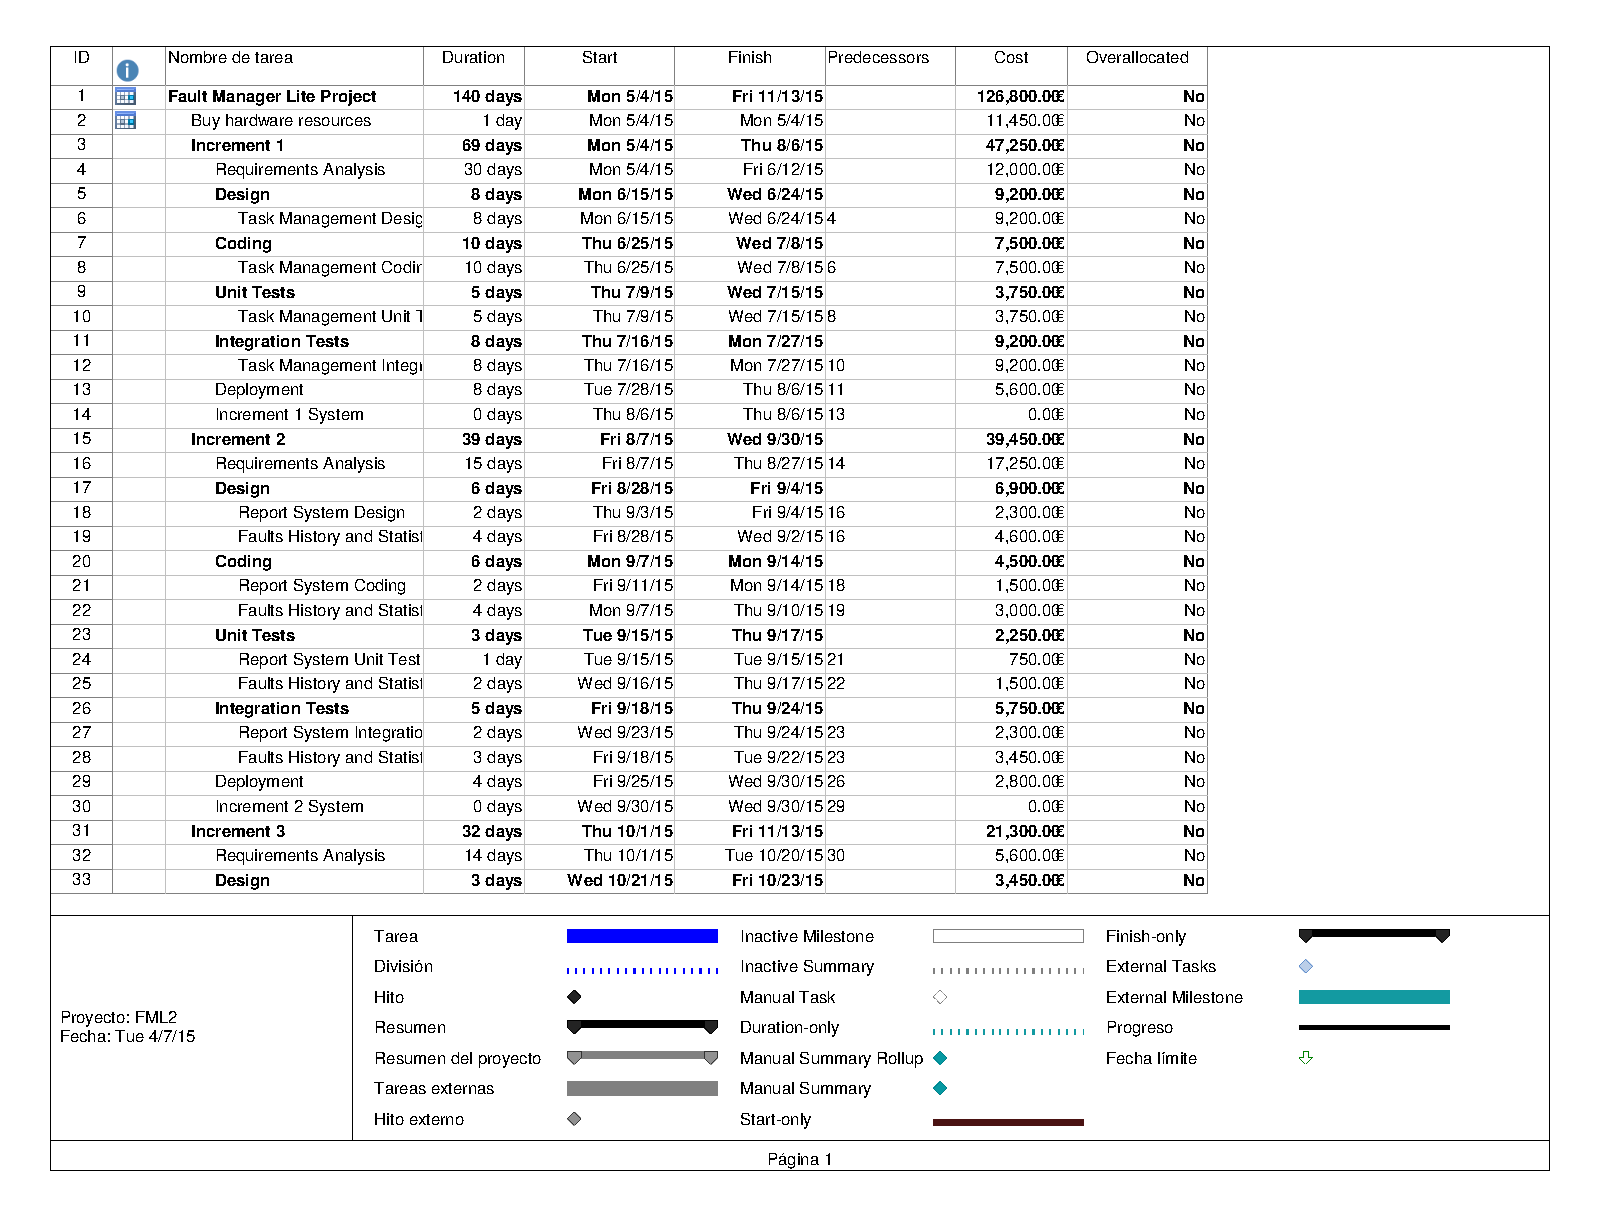
\includepdf[scale=0.8, pages={1-}, nup=1x2, pagecommand={}]{Project.pdf}

\end{document}
